\subsection{Fit method}
\label{sec:swave:meas:fitmethod}

The measurement of \FS was obtained from a measurement of the \kpi mass spectrum for \BdToKpimm events.
%The main issue with this method is that there are both non-resonant \kpi, \kpi S-wave and \kpi P-wave events in the 
%signal and in the background region.
%The second issue is that due to this uncertainty on the exact model for the background, the 
% model constructed in the previous section has a large number of empricially determined parameters.
In order to obtain a reasonably accurate fit by minimising the number of free parameters to fit the \mkpi distribution, % to the \kpimm and \kpi mass distribution of \BdToKpimm events, 
 a multiple stage fit was used to constrain the parameters of the \Bd mass shape before the angular distribution is fitted.
The \kpimm mass spectrum, which is independent of the \kpi spectrum for the small \psq region considered, was used to determine 
the  total fraction of signal and background in each of the \qsq bins.
Once the signal fraction was fixed the \kpi line shape was subsequently fitted to obtain the value of \NS.
This allows the S-wave fraction, \FS, to be calculated from the integration of \FSi and \FPi in the \kpi region from 0.64 to 1.00\gevgevcccc.

\subsubsection{Constraining the \mkpimm mass}

The first part of the fit strategy was to constrain the mass distribution using selected \BdToJpsiKpi data. 
This high statistics sample of around 200k events allows the parameters for the double Crystal Ball model to be precisely constrained.
There is an additional contribution from \BsToJpsiKpi which is suppressed by several orders of magnitude compared to \BdToJpsiKpi but still has to be taken into account.
The method is the same  as was used to constrain the parameters of the two Crystal Ball functions in Section~\ref{sec:kstmm:resextraction}.
The result of the fit of the mass model to the \BdToJpsiKpi data is shown in Fig.~\ref{fig:swave:meas:jpsikstar:fit}.
\begin{figure}[tbp]
\centering
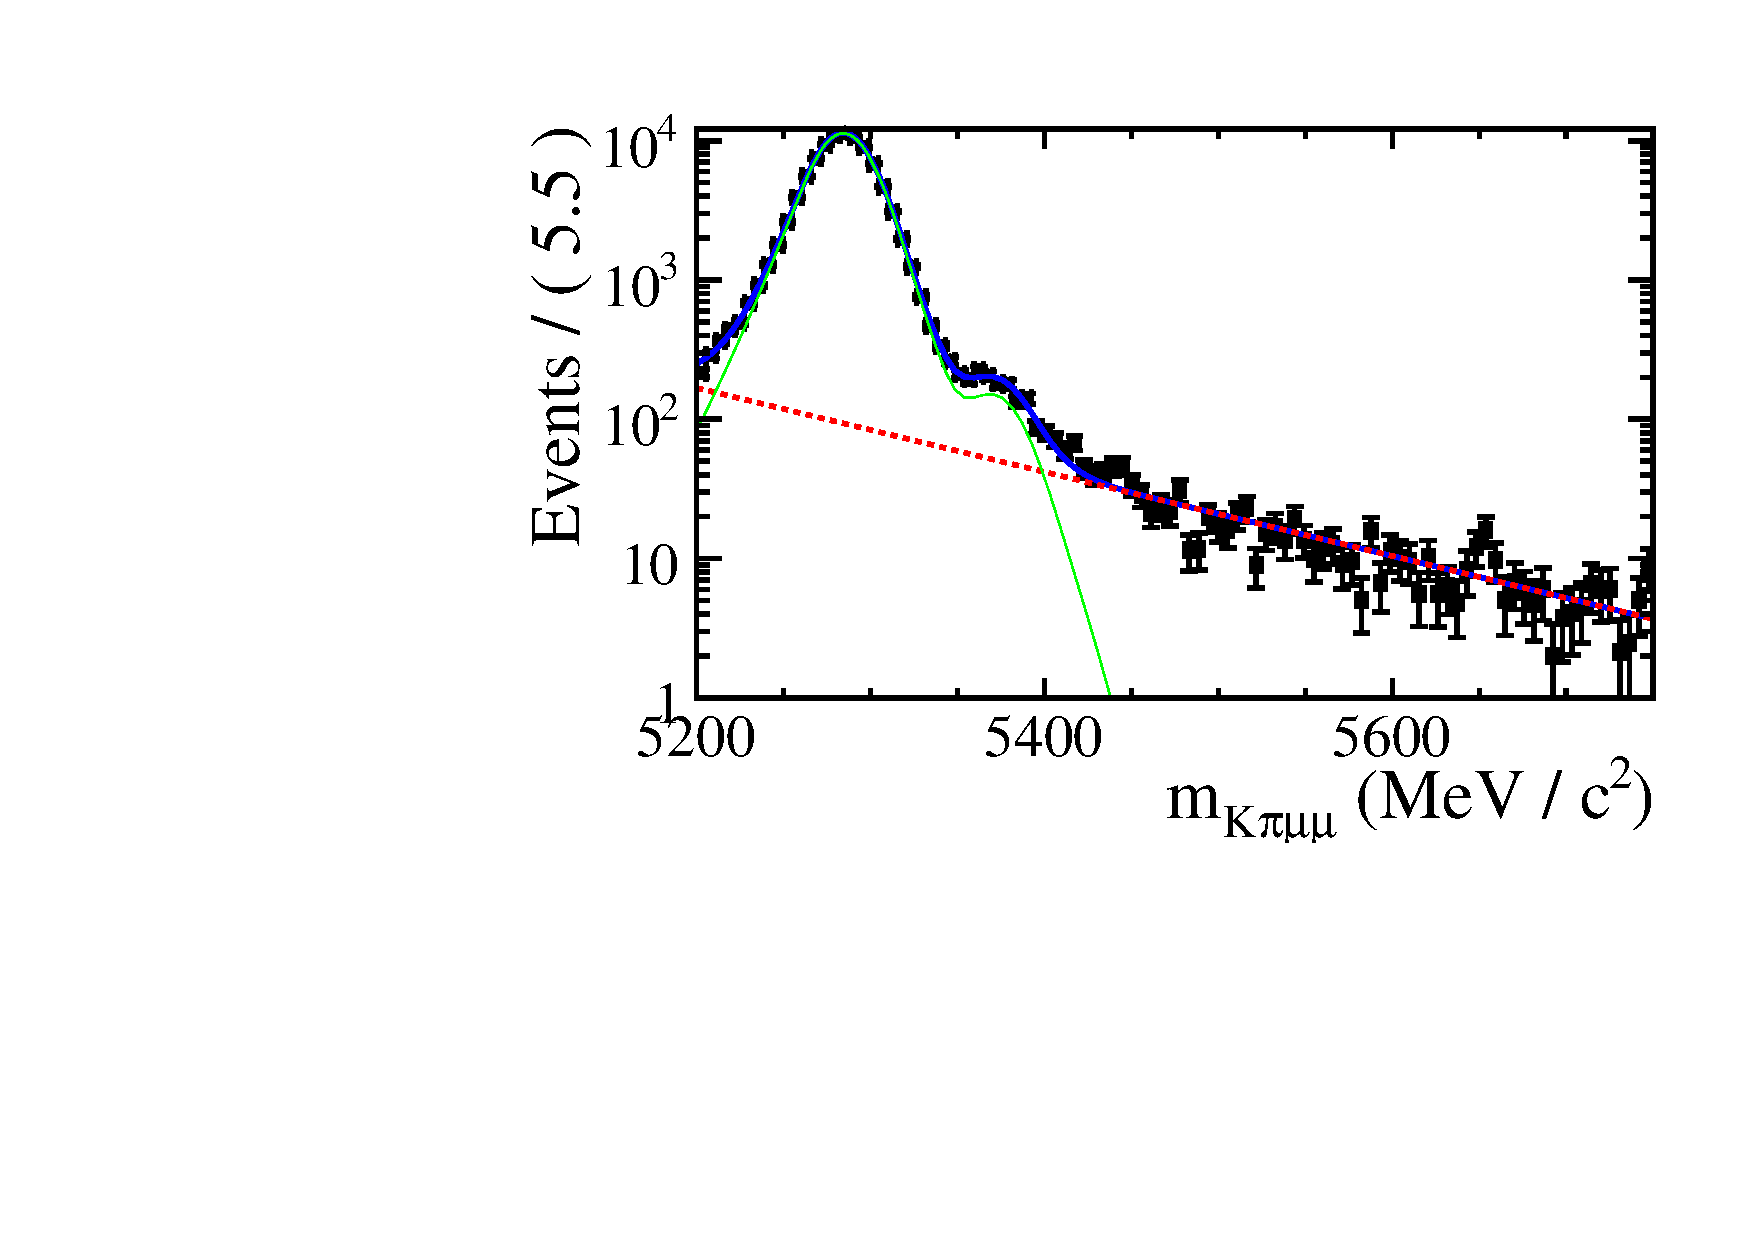
\includegraphics[width=0.48\columnwidth]{chapter7/figs/fit_jpsikstar_mass_fit_logy.pdf}
\caption[ The fit to selected \BdToJpsiKpi data with the model for the \kpimm distribution.  ]
{The fit to selected \BdToJpsiKpi data with the model for the \kpimm distribution. 
It is possible to see a contribution from \BsToJpsiKpi to the right of the \BdToJpsiKstar peak.
There are $115900\pm350$ \BdToJpsiKpi signal events. 
The total PDF is given in \textcolor{blue}{blue}, the signal component in \textcolor{green}{green} and the background component is the \textcolor{red}{red} dashed line.
~\label{fig:swave:meas:jpsikstar:fit} }
\end{figure}
It can be seen that the double Crystal Ball model results in a good fit to the signal peak and the \BsToJpsiKpi contribution. 
The values of the signal parameters from this fit are fixed to their values and the value of the background parameter is ignored.
%This is because there is a different distribution of background events in the \BdToJpsiKpi and in \BdToKpimm as shown in Fig.~\ref{fig:swave:mass:mkpi}.

In order to obtain a complete description of the \kpimm mass spectrum for the \BdToKpimm data,
for each \qsq region the data was fitted with the fixed signal model allowing  the background parameter and the the total fraction of signal to vary.
The results of both these fits allow the fraction of signal, $f_S$, to be constrained for the fit to the \kpi mass distribution.

\subsubsection{Fitting the \kpi mass distribution}

The proportion of \kpi S-wave to P-wave, \NS, in each of the \qsq bins was determined by fitting the \kpi mass distribution to the data.
In order to constrain the number of remaining parameters, several assumptions were made about both the signal and background model for the \mkpi spectrum.
This is a simpler model than the one described in Chapter~\ref{chap:swave:theo} but the only one possible 
given the low statistics in data and the reduced accuracy of the acceptance correction.

There are three sets of parameters for the \mkpi signal models: the parameters for the P-wave, the resonant S-wave and the non-resonant S-wave.
The parameters describing the \Kstarzo are well known and can be constrained to the values given in Ref~\cite{PDG2012}.
The parameters for the non-resonant part of the \Kstarzz model are left free in the fit and their starting values are taken from Table~\ref{tbl:params}.
The parameters for the resonant $\Kstarzz(1430)$ are constrained to the values given in Ref~\cite{PDG2012}.
The phase difference between the S-wave and the P-wave is integrated out.

The background distribution in \mkpi is not known a priori but it can be assumed that there is an increase from the \kpi threshold due to the phase space available.
Reasonable ranges for the parameters for the empirical \mkpi background function were obtained through fits to the \kpi mass spectrum using events with a \mkpimm of greater than 5400\mev.
This assumes  that these events with high \kpimm masses can be used to model the \mkpi background spectrum.
This was checked by fitting the background in the \Bd signal window with the same empirical background model.
%From these fits, it is possible to obtain the number of background events in the \Bd mass window and above the \Bd mass window.
The distribution of \BdToKpimm background events in the \Bd signal region and above the \Bd signal region are shown in Fig.~\ref{fig:swave:background:dist}.
\begin{figure}[tbp]
\centering
\subfigure[]{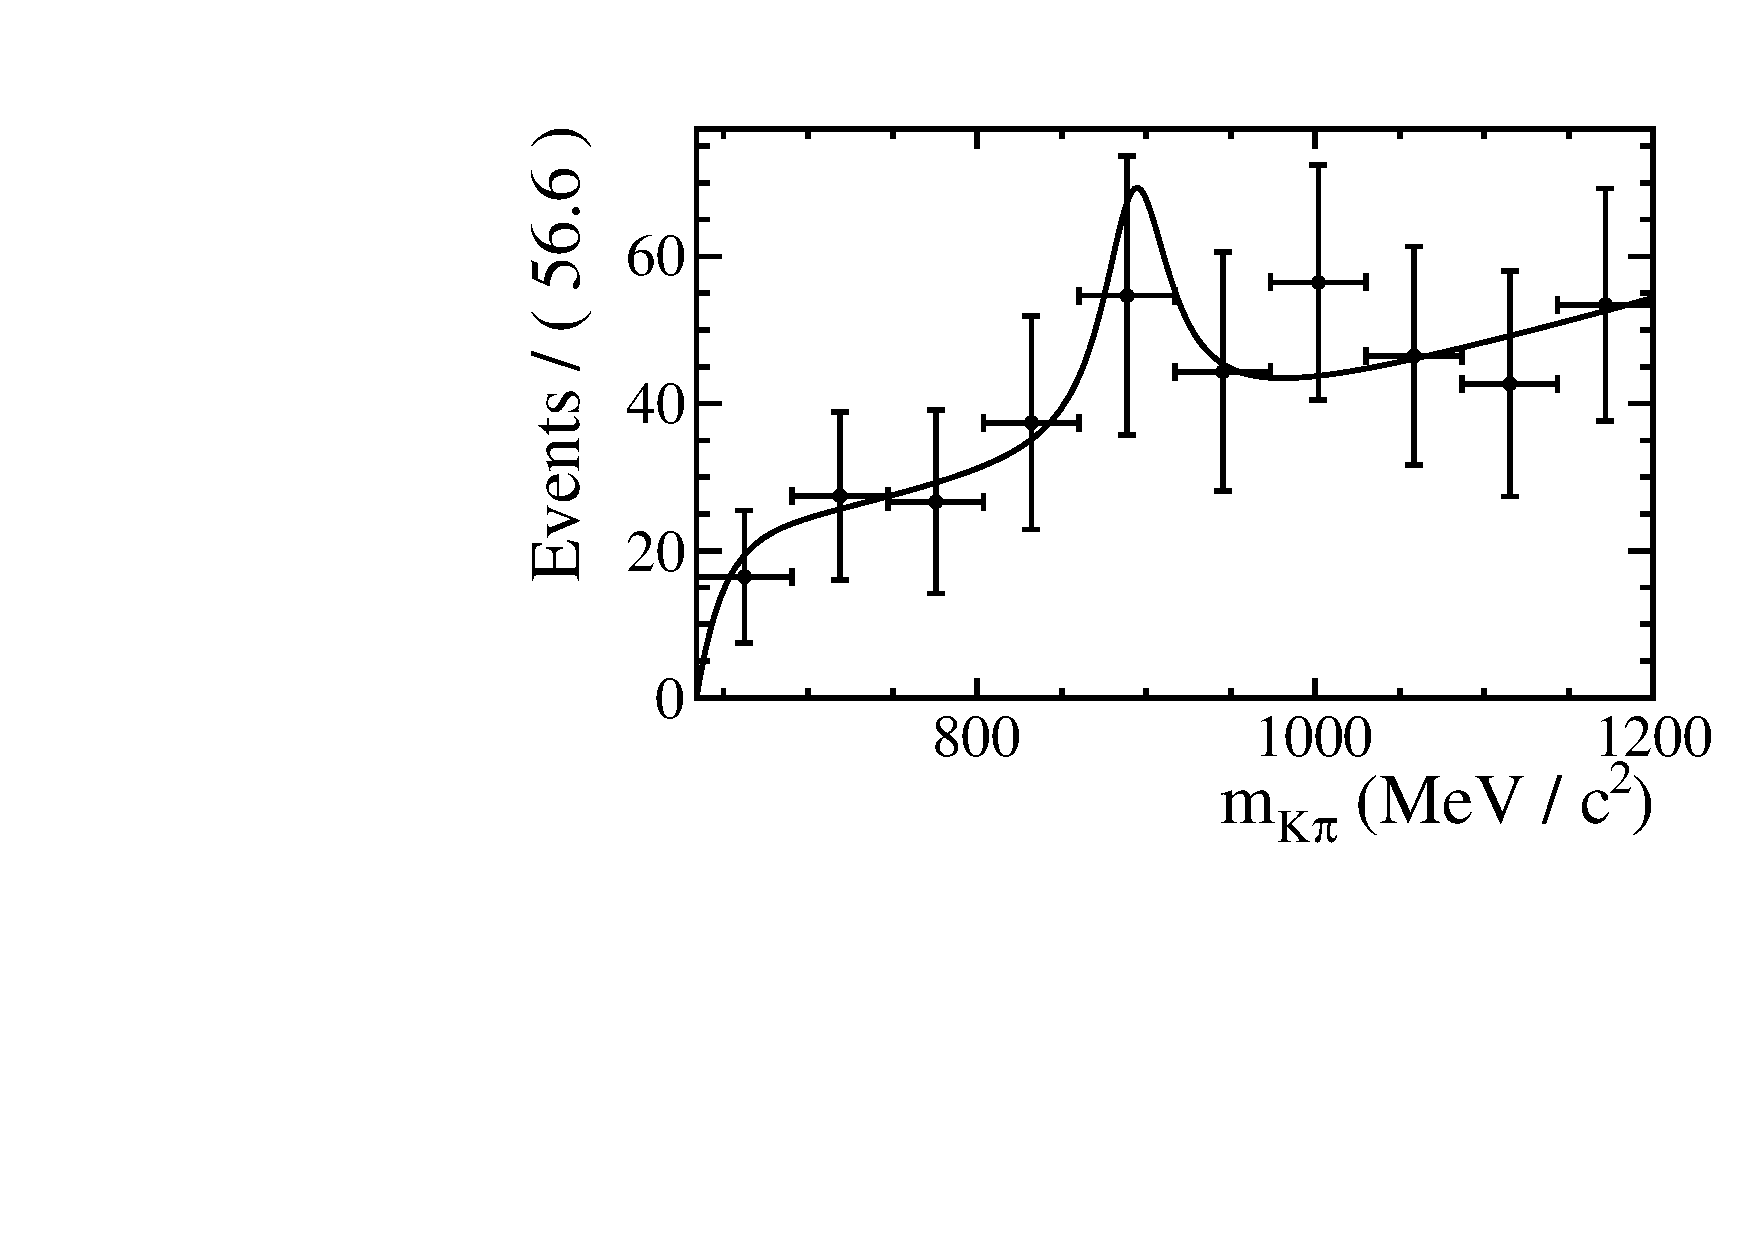
\includegraphics[width=0.48\columnwidth]{chapter7/figs/bkg/kstarmumu_fit_bkg_10.pdf}}
\subfigure[]{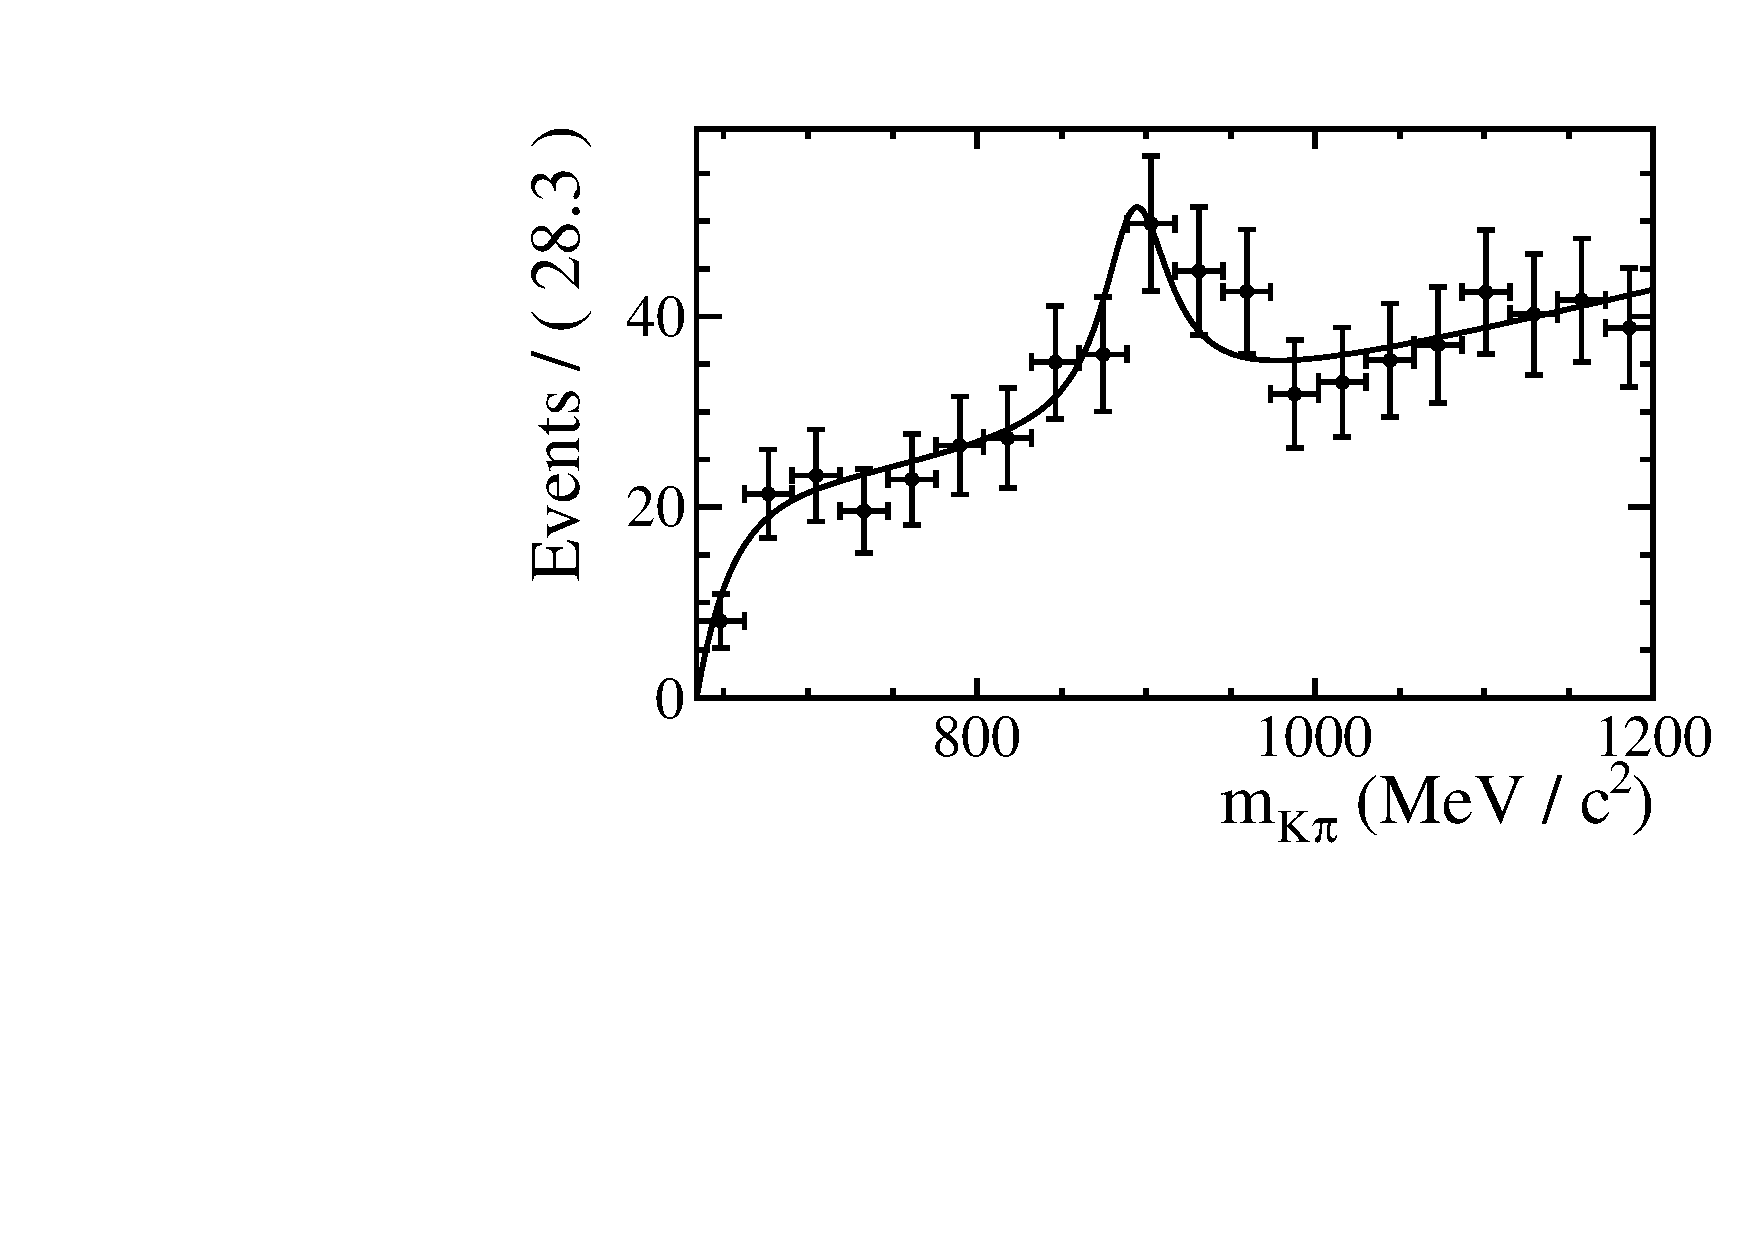
\includegraphics[width=0.48\columnwidth]{chapter7/figs/bkg/kstarmumu_fit_bkg_upper_20.pdf}}
\caption [ The distribution of background events in bins of the \kpi mass in (a) the region from 5200 to 5400\mevcc and (b) above 5400\mevcc. ]
{ The distribution of background events in bins of the \kpi mass in (a) the region from 5200 to 5400\mevcc and (b) above 5400\mevcc.
It is possible to see an increase in the background distribution from threshold for both regions. 
The background distributions are fitted with the empirical function in Eq~\ref{eq:swave:mkpi:background}.
The background in the \Bd signal region is obtained from extended maximum likelihood fits to the \Bd mass in 10 bins of \mkpi.
 ~\label{fig:swave:background:dist} }
\end{figure}
It is possible to see that the background increases from threshold and there is a small contribution from a \kpi P-wave state of around 5\%.
%These fits were only used to obtain the starting values for the background parameters in order to not use the same information twice.
The final fit model contains the S-wave proportion, \NS, along with the signal and background model parameters for the \kpi mass spectrum as free parameters.
In the case of the fit model converging to a limit of zero S-wave contribution, the Feldman-Cousins technique~\cite{PhysRevD.57.3873} was used to calculate a 95\% upper limit on the value of \FS.

\subsection{Determination of \FS}

Once the constrained model has been applied to the data, the proportions of S-wave and P-wave were calculated by integration over \mkpi from 0.64 to 1 \gevgevcccc.
The fraction of the S-wave in the P-wave resonance region was calculated by integrating Equation~\ref{eq:swave:meas:sig:swave},
to give the differential branching fraction in terms of \psq and \qsq, 
\begin{align}
\label{eq:swave:meas:sig:dbr}
\frac{1}{\Gamma^{''}} \frac{\text{d}^3\Gamma}{\text{d}\qsq\text{d}\psq} &=  \FSi(\psq,\qsq) + \FPi(\psq,\qsq)
\end{align}
so the S-wave fraction integrated over \psq and \qsq is given by
\begin{align}
\label{swave:fscalc:int}
\FS &=  \frac{ \int \FSi(\psq,\qsq) \text{d}\psq\text{d}\qsq }{ \int \left[ \FSi(\psq,\qsq) + \FPi(\psq,\qsq) \right] \text{d}\psq\text{d}\qsq } \, .
\end{align}

